To estimate the effect, we use data on GDP, government spending, and government revenue from FRED between 1960Q1 and 2007Q4. The upper end of the estimation window is chosen due to changes in growth trends post-2008, though we believe with a more robust detrending procedure we would observe similar business cycle effects during the post-2008 period \parencite{benigno2018stagnation}.

\begin{figure}[t!]
    \centering
    \caption{Detrended data series for GDP, government spending, and government revenue}
    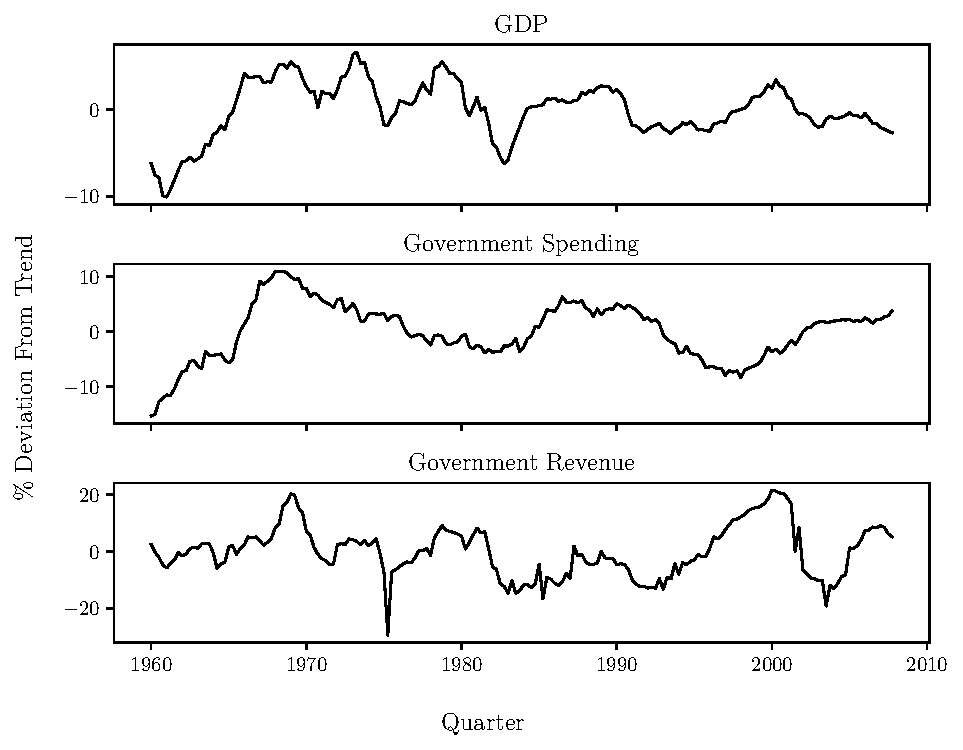
\includegraphics{figures/detrended_data.pdf}
    \label{fig:dta}
\end{figure}

We use the ``Gross Domestic Product" series for GDP, ``Government Consumption Expenditures and Gross Investment'' series for government spending, and ``Federal Government Current Tax Receipts'' series for government revenue. Each series is then divided by the GDP Deflator to convert it to real terms instead of nominal, then detrended according to the procedure in \ref{subsec:detrend}. Detrended series throughout the period are shown in Figure \ref{fig:dta}.
